\subsection{Abschirmung}

\begin{figure}[!h]
	\centering
	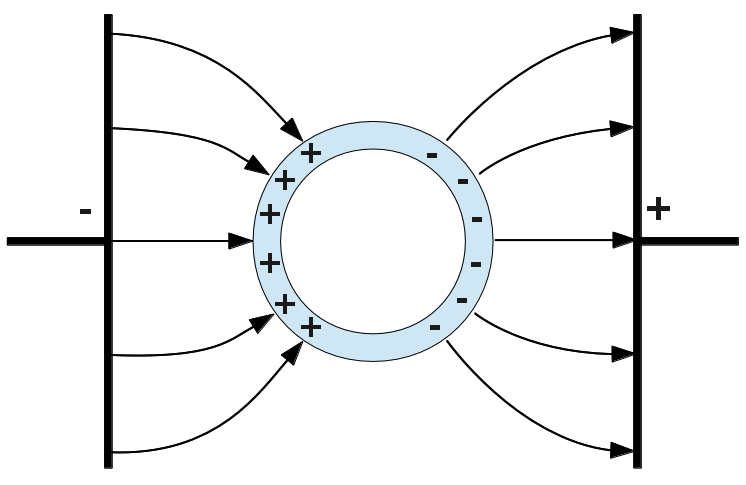
\includegraphics[width=\textwidth]{RingEFeld}
	\caption{Abschirmung eines elektischen Feldes durch einen Metallring}
	\label{fig:abschrimung}
\end{figure}

In einem zweidimensionalen elektrischen Feld kann durch einen geschlossenen Ring aus Metall ein elektrischen Feld abgeschirmt werden. Dies passiert, da die beweglichen negativen Ladungen im Metallring zur positiven Seite des äußeren Feldes wandern (entgegen der Feldlinien) und auf der anderen Seite des Ringes ein positive Ladung hinterlassen. Diese Ladungstrennung führt ihrerseits zum Aufbau eines elektrischen Feldes, welches in die entgegengesetzte Richtung zeigt und das \glqq äußere\grqq{} Feld im Inneren des Rings neutralisiert.\endnote{\glqq Abschirmung eines E-Feldes\grqq{} von Till Blaha - Eigenes Werk. Lizenziert unter Gemeinfrei.}

Im dreidimensionalen Raum ist dafür eine Hülle nötig, die man dann \glqq Faradayischer Käfig\grqq{} nennt.